\documentclass{pj}
\usepackage{graphicx}

%\usepackage{mwe}
\usepackage{subcaption}
\captionsetup{compatibility=false}
\usepackage{textcomp}
\usepackage{float}

\usepackage{array}
\newcolumntype{P}[1]{>{\centering\arraybackslash}p{#1}}
\newcolumntype{M}[1]{>{\centering\arraybackslash}m{#1}}
\usepackage[labelfont=bf]{caption}

\begin{document}
\setcounter{page}{1}
\pjheader{Vol.\ x, y--z, 2014}


\title[Design of Radiated Comb Generator]
{Design of Radiated Comb Generator Using Positive Emitter Coupled Logic (PECL) D Flip-Flop}
\footnote{\it Received date}  \footnote{\hskip-0.12in*\, Corresponding author:~Yoppy (yoppy.chia@gmail.com).}
\footnote{\hskip-0.12in\textsuperscript{1} Research Center for Quality System and Testing Technology - Indonesian Institute of Sciences (P2SMTP--LIPI). \textsuperscript{2} The second affiliation.}

\author{Yoppy\textsuperscript{*, 1} and Muhamad~Imam Sudrajat\textsuperscript{1}}


\runningauthor{Yoppy and Sudrajat}

\tocauthor{FistName1~LastName1 and FistName1~LastName1}

\begin{abstract}
Comb generator has been an indispensable tool in the electromagnetic compatibility (EMC) testing field. It is used for calibration and self checking for EMC testing systems. Existing radiated comb generators are usually implemented using step recovery diodes (SRD), Schottky diodes, transistors, etc. This paper presents a rarely explored yet promising radiated comb generator that makes use of PECL D Flip-Flop as the pulse forming component. PECL is one of the fastest in logic gates families, whose switching rate goes into sub nanosecond range. The D Flip-Flop is not used conventionally in the sense of usual digital circuits. Instead, its asynchronous reset feature is purposefully exploited such that at each rising clock a very short pulse is produced on the output. Measurements show that the generated pulses typically possess fall time and rise time of 330ps and 410ps respectively. Its frequency accuracy is offset by +24 ppm, which is common for crystal oscillators. When connected to a monopole rod antenna, the comb generator is able to generate radiated emissions that have smooth envelope profile up to 1000 MHz frequency range as measured in 3m semi anechoic chamber.
\end{abstract}

%\mytableofcontents
%\tableofcontents

\setlength {\abovedisplayskip} {6pt plus 3.0pt minus 4.0pt}
\setlength {\belowdisplayskip} {6pt plus 3.0pt minus 4.0pt}

\

\section{Introduction}
\label{sect:introduction}

A comb generator is basically a periodic pulse generator. When viewed from frequency domain, such pulse train is represented by the fundamental frequency and its multiple harmonics. When observed from the time domain, the pulse duty cycle and frequency dictate the spectrum profiles in  the frequency domain. In general smaller duty cycle, which is characterized by shorter pulsewidth and also faster rising and falling times, generates smoother and higher frequency spectrum profiles. 

Radiated comb generator, also known as radiation source, has been an important tool for electromagnetic compatibility (EMC) laboratories to ensure the quality of measurement results. Calibration is usually performed in the interval of one or two years. However in between calibration periods, frequent intermediate checks should be carried out to identify if there is any irregularities in measurement results. Also, self-check is also necessary when there is replacement of connectors, cables, or equipements. For practical reasons, comb generator is an essential tool in performing intermediate checks because it is usually portable, battery operated, and able to generate multiple frequencies simultaneously in the whole measurement frequency range.

Radiated comb generator essentially consists of periodic pulse generator and radiating elements. For EMC applications the frequency range covers from 30 MHz up to 1, 2, 5 or 6 GHz, depending on the highest internal frequency of the unit under test \cite{IEC2015}. There are several ways to produce periodic pulses, for example using discrete silicon RF transistor, step recovery diode (SRD), tunnel diode, non linear transmission line (NLTL), etc \cite{JamesRAndrews2008}. Pulse generators based on SRD and Schottky diode techniques are able to generate a pulse width of a few hundred picoseconds \cite{Miao2003}\cite{Zhou2015}\cite{Maxwell2008}.  Another method exploiting differential AND gates of emitter coupled logic (ECL) devices shows that a pulse width of approximately 1 ns can be produced \cite{15259}. 

In low cost designs, a radiated comb generator producing periodic square waves has been constructed using inverter gates of TTL device \cite{Dau-Chyrh2013}. It is shown that the frequency peaks have fluctuant spectrum envelope profiles. This can be explained by the fact that the comb generator makes use of square waves instead of short pulses, and also TTL devices have relatively slow rising/falling edges (2-10 ns) \cite{Montrose1999}. Another design of comb generator using NAND gates also exhibits similar jagged spectrum envelope profiles \cite{Ungvichian2006}. However for ease of use purposes  it is highly desirable that all the frequency peaks form a smooth profile.

Another simple and cost effective design of pulse generator employing CMOS D Flip-Flop 74AC74 is described in \cite{Martin1988}. Although the generated pulse width is limited to about 6 ns, the ingenious design can be adapted to produce narrower pulses by using faster logic devices. In this paper, a comb generator using single-ended positive ECL D Flip-Flop is proposed. Among logic families, ECL technology is one of the fastest devices whose switching edges go below a nanosecond \cite{Montrose1999}. Unlike differential ECL, single-ended PECL is simpler to implement and uses fewer component counts. The realized comb generator comprises a pulse generator board and a monopole rod antenna. Measurements and evaluation in time domain as well as frequency domain are presented. 

\section{Implementation}
This paper aims to design a simple and low cost radiated comb generator useable up to 1 GHz range. The comb generator consists of two main parts, i.e. a periodic pulse generator and a radiating element. The pulse generator implementation is based on a single-ended positive emitter coupled logic D Flip-Flop (PECL DFF). Due to its simplicity, monopole rod antenna is employed as the radiating element.


\begin{figure}[h]
	\centerline{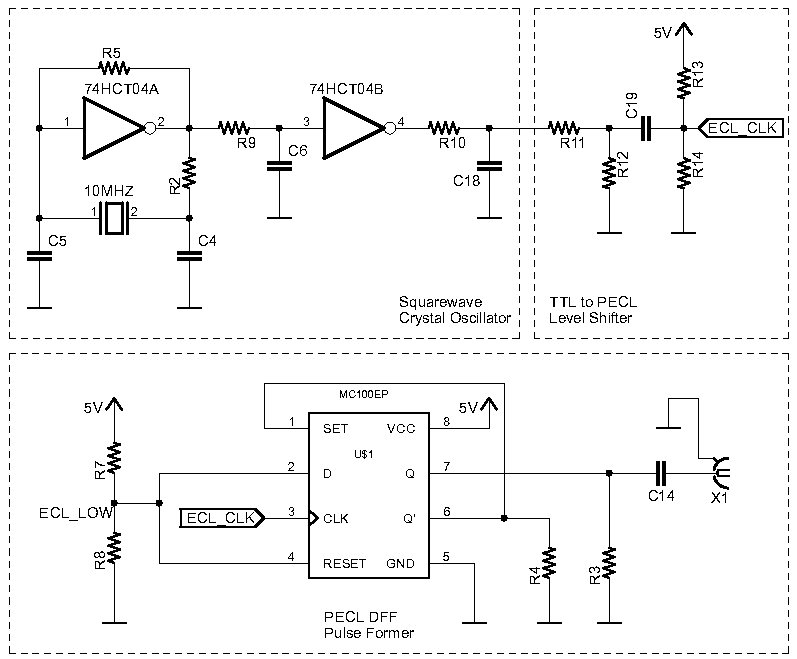
\includegraphics[width=0.75\columnwidth,draft=false]{comb_schematic.pdf}}
	\caption{Schematic of PECL DFF based pulse generator}
	\label{fig:pulse_generator}
\end{figure}

As shown in Figure~\ref{fig:pulse_generator}, the pulse generator is powered at 5 volts, and consists of three main parts, i.e. square wave oscillator, TTL to PECL level shifter, and PECL DFF pulse former. The square wave oscillator is constructed from 74HCT04 TTL-compatible CMOS inverter and a 10 MHz crystal. R9, R10, C6, and C18 function as ringing filters at the inverter's output. Unless damped, the ringing could disrupt power supply lines and eventually propagates to next stages in the circuit. As a result, the final pulse output may  become deteriorated. The square wave has a TTL voltage level where a LOW is at 0 volts and HIGH is 5 volts. However positive ECL (PECL) has different voltage level definitions where 3.2 volts is a LOW and 4.0 volts is a HIGH. Therefore, TTL square waves need to be converted to ECL level before fed to the MC100EP DFF. MC100EP has a truth table as shown in Table~\ref{tab:truth-mc100ep} \cite{Semiconductor2008}. 


\begin{table}[h]
	\renewcommand{\arraystretch}{1.3}
	%\captionsetup{justification=centering}
	\caption{Truth table of MC100EP DFF}
	%\vskip0.2in
	\begin{center}
		\small \begin{tabular}{|M{1.7cm}|M{1.7cm}|M{1.7cm}|M{1.7cm}|M{1.7cm}|}\hline
			\textbf{D} & \textbf{SET} & \textbf{RESET} & \textbf{CLK} & \textbf{Q}  \\ \hline
			L & L   & L     & ${\uparrow}$   & L \\ \hline
			H & L   & L     & ${\uparrow}$   & H \\ \hline
			X & H   & L     & X   & H \\ \hline
			X & L   & H     & X   & L \\ \hline
			X & H   & H     & X   & UNDEF \\ \hline
			
		\end{tabular}
	\end{center}
	\label{tab:truth-mc100ep}
\end{table}
 
Referring to Figure~\ref{fig:pulse_generator}, D and RESET are always held LOW. Incoming rising edge at CLK input causes Q become LOW and $\overline{Q}$ transit HIGH. Because $\overline{Q}$ output is tied to SET input, when $\overline{Q}$ is going HIGH, then Q is forced to HIGH immediately irrespective of the CLK input. Q then stays at HIGH state until the next rising edge of the CLK input. As a result of such an abrupt SET action, a very short downward pulse is generated at Q output. Therefore periodic downward pulses are produced at each rising edge of the clock. C14 is used to filtered out the DC component so that the net result is a negative pulse on the RF connector output. 

\begin{figure}[h]
	\centerline{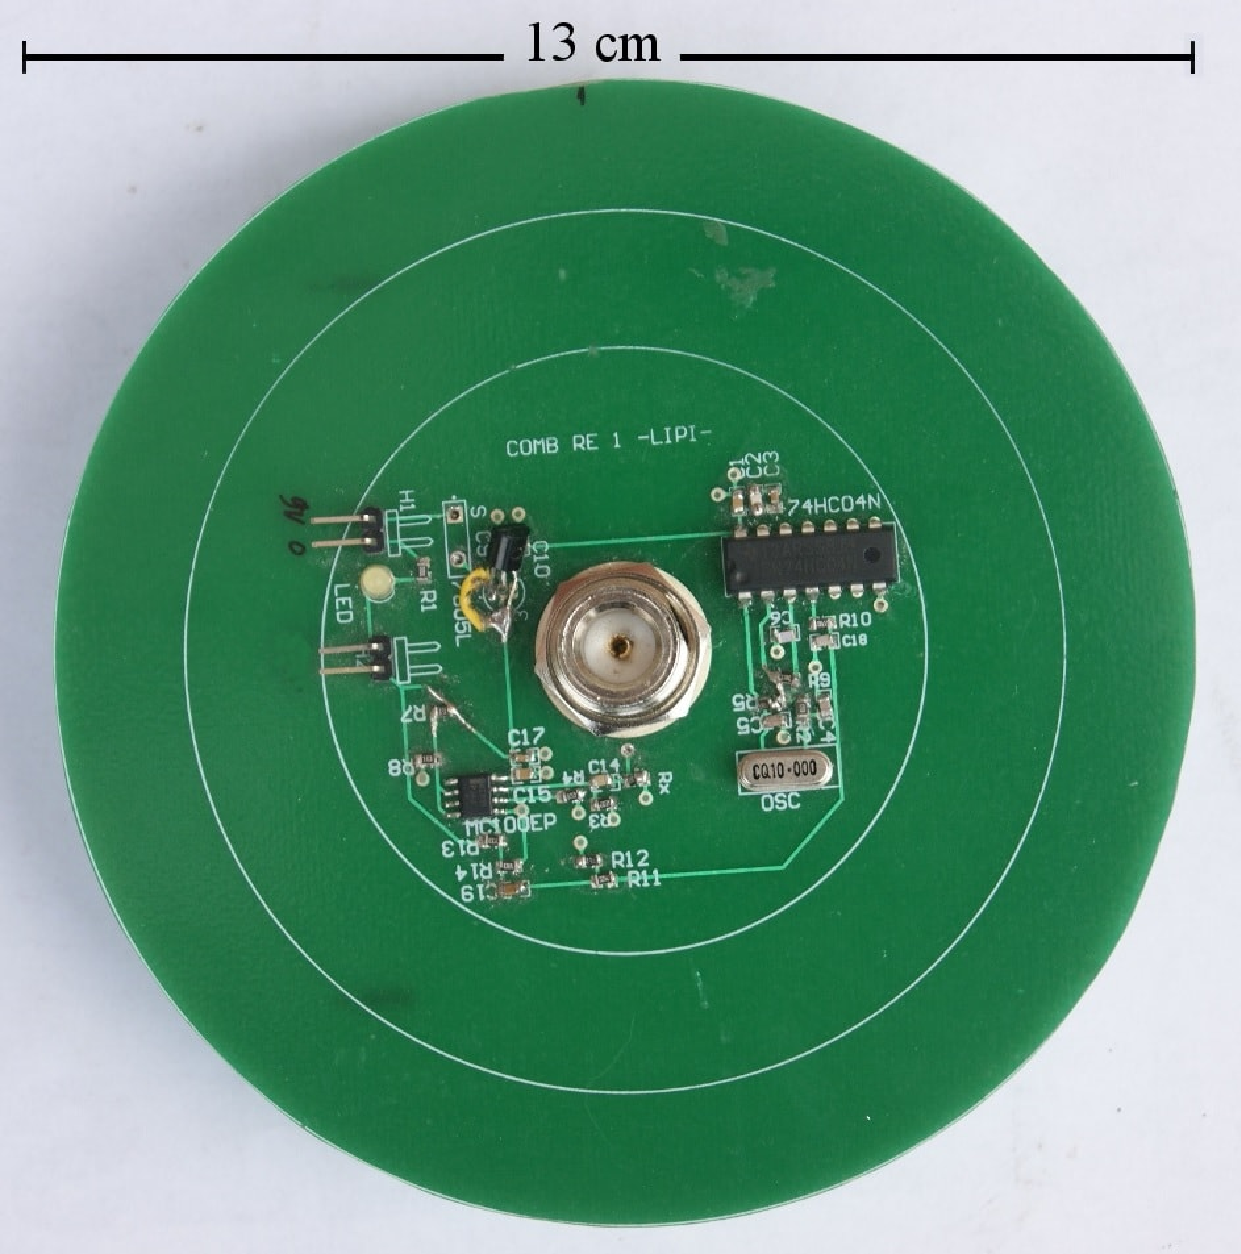
\includegraphics[width=0.55\columnwidth,draft=false]{board_comb_re.pdf}}
	\caption{Printed circuit board of pulse generator}
	\label{fig:board_comb_re}
\end{figure}

Figure~\ref{fig:board_comb_re} depicts the pulse generator printed circuit board. It has a diameter of 13 cm, and has a solid copper on the bottom layer functioning as a ground plane. The female N connector located in the center of the board serves as the antenna holder. For simplicity purposes, the antenna is made of a copper rod that has a diameter of 1.7 mm and a length of 30 cm, and it fits in the signal pin of the N connector. It is effectively a simple monopole antenna. 


\section{Evaluations}


\subsection{Time Domain}

Frequency spectrum produced by comb generator is directly related to the generated pulse repetition as well as pulse shape in the time domain. It is known that pulse repetition rate translates to the frequency spacing in the frequency spectrum. Whereas pulse shape determines the spectrum envelope profile. To obtain flat and smooth envelope across wide frequency range, the pulse width should be as short as possible. Pulse width measurement is done using Agilent 3 GHz DSO80304B oscilloscope, which has capability of measuring rise time and fall time up to 140 ps \cite{agilent_dso80000}. Figure~\ref{fig:comb_re_pulse_out} shows the typical pulse shape measured at the comb generator RF output. It has a fall time and  and rise time equal to 330ps and 410ps respectively.

% Figure: pulse shape measured from oscilloscope
\begin{figure}[h]
	\centerline{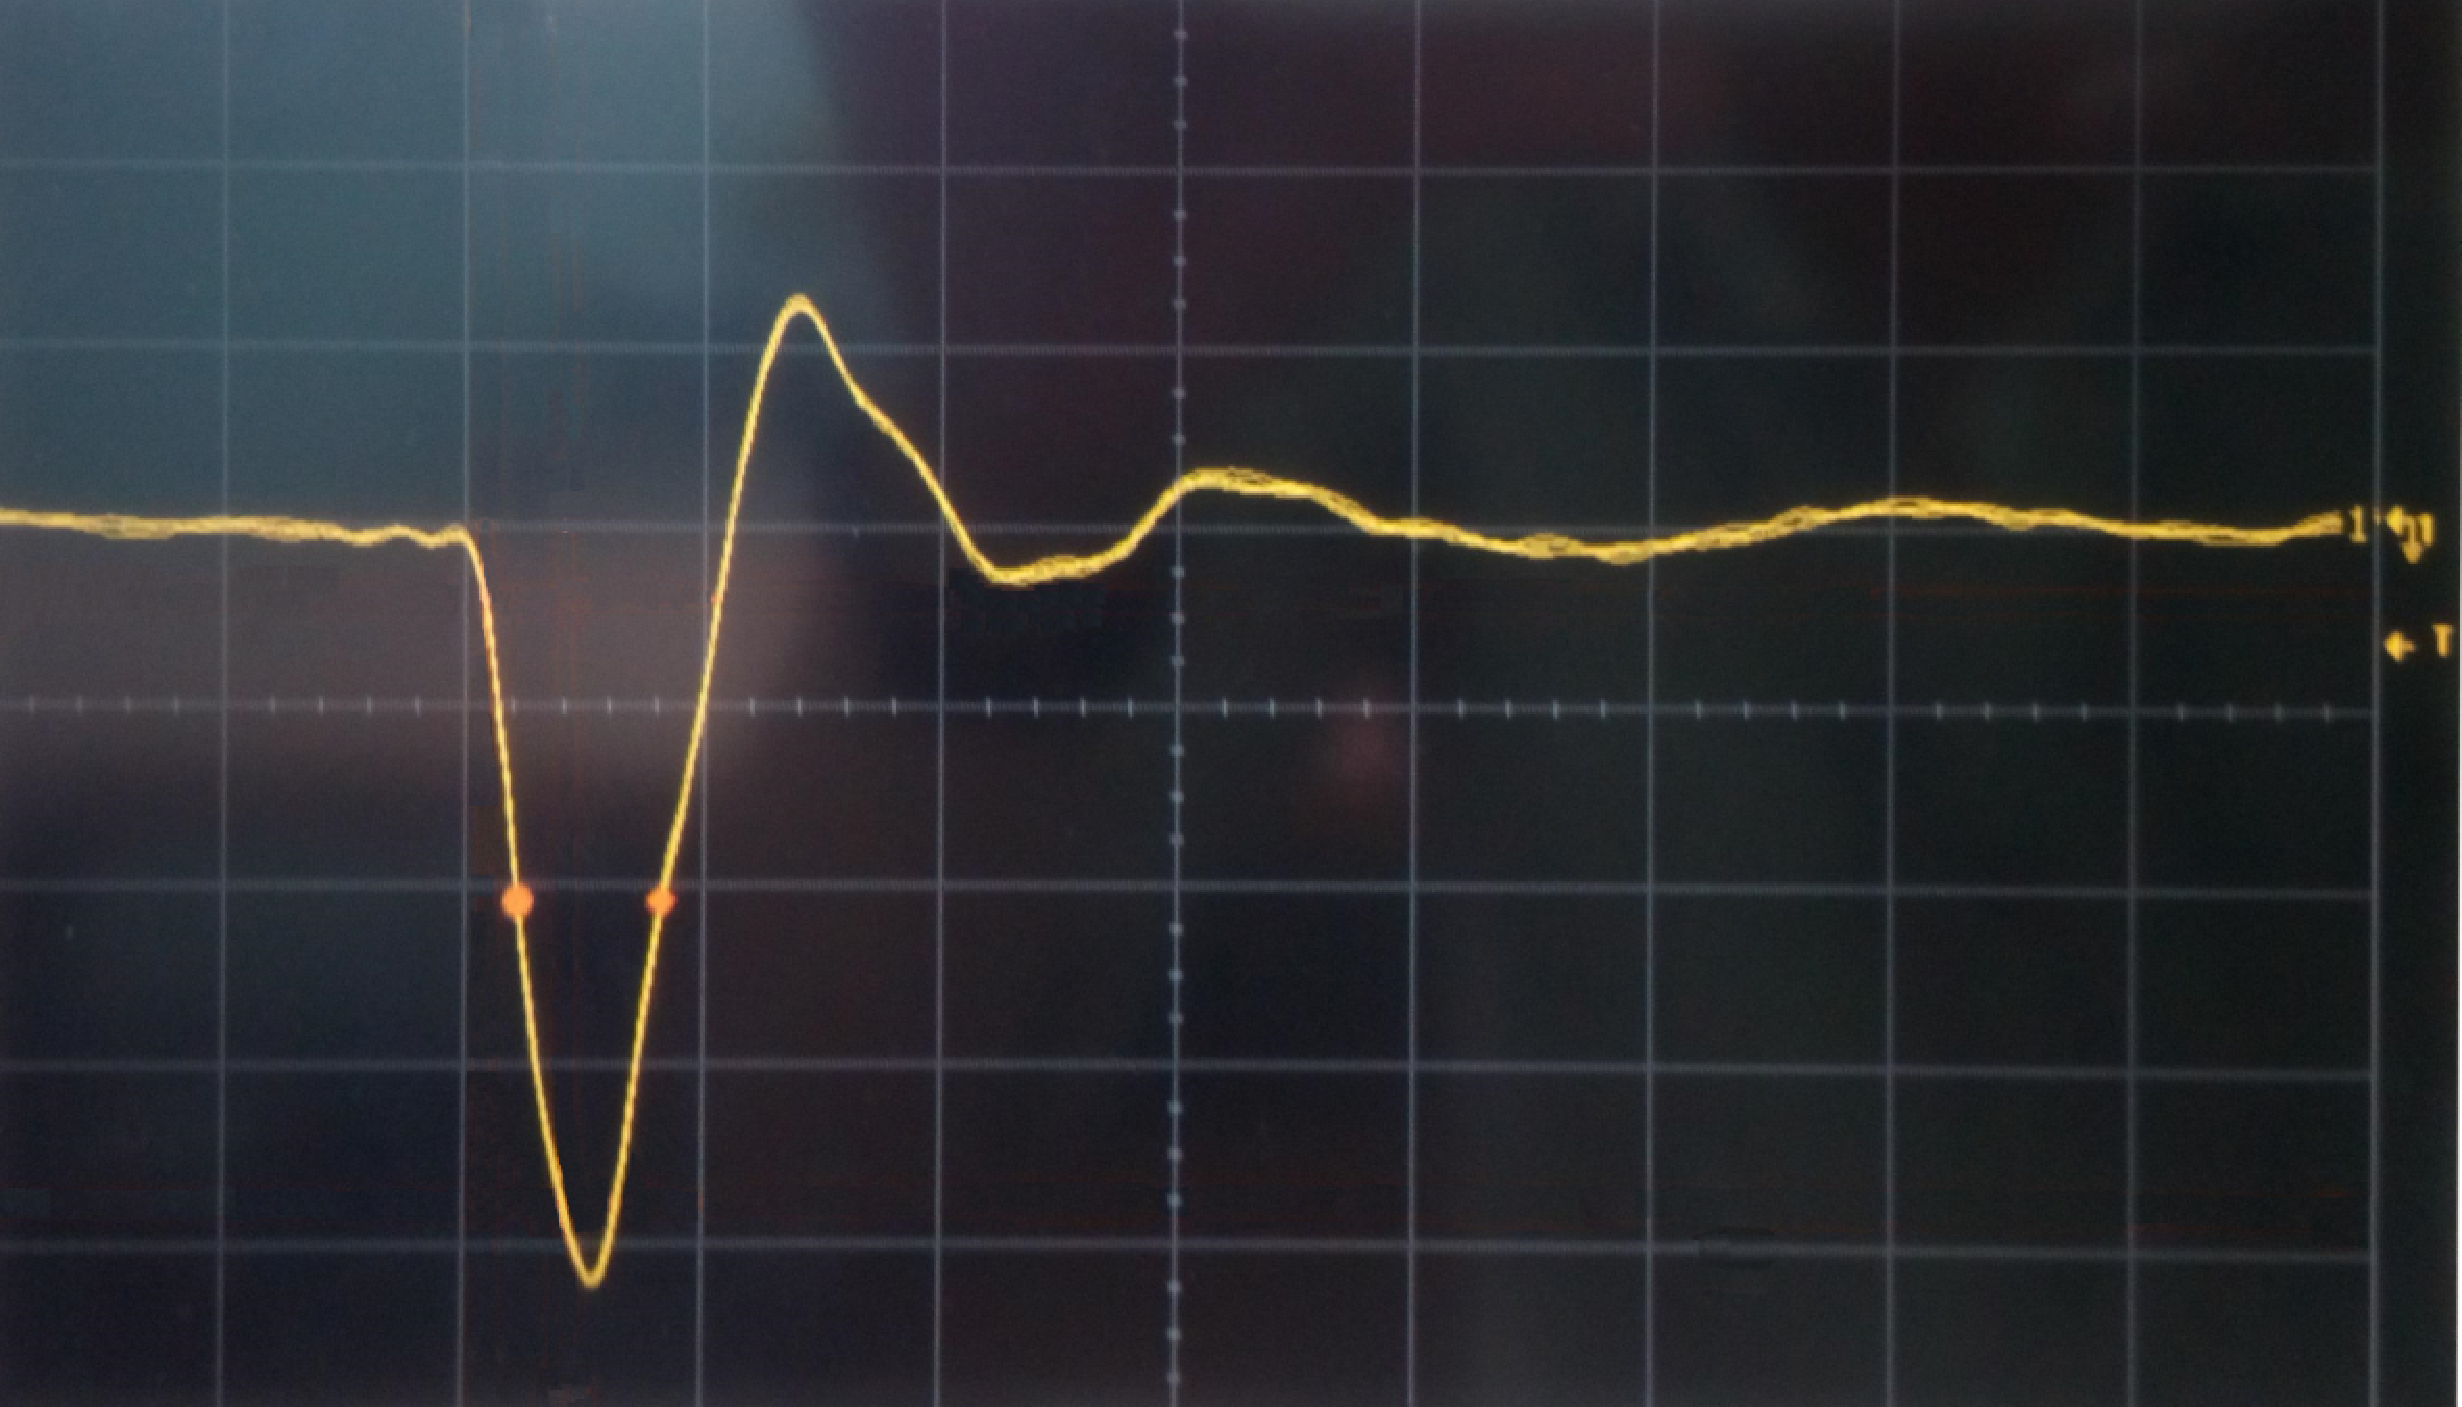
\includegraphics[width=0.6\columnwidth,draft=false]{comb_re_osc_out_2.pdf}}
	\caption{Typical pulse shape measured at the board RF output (1 ns/div, 200 mV/div)}
	\label{fig:comb_re_pulse_out}
\end{figure}

\subsection{Frequency Domain}

Measurements in the frequency domain are done in two methods, i.e. direct measurement and radiated emission measurement in a 3 meter semi anechoic chamber (SAC). In the former, the comb generator is directly connected to a spectrum analyzer, whose measurement results depicted in Figure~\ref{fig:comb_re_direct}. It does not show a straight flat profile in the whole frequency range, which might be explainable by the fact that the pulse shape in Figure~\ref{fig:comb_re_pulse_out} shows some amount of overshoot and ringing.  However, in general it still exhibits a smooth profile and stands out from the noise floor. It can be reported that the frequency accuracy is offset by +24 ppm. This is a typical figure obtainable from crystal oscillators. In order to achieve higher accuracy, temperature compensated crystal oscillator (TCXO) or oven-controlled crystal oscillator (OCXO) can be used instead.

Meanwhile, measurements in SAC follows a standard radiated emission test procedure. The comb generator (pulse generator with monopole antenna) is placed on a 80cm high non-metallic rotating table and is movable from 1m to 2m above the ground. A measuring BicoLog antenna is located 3m away from the rotating table. Since the comb generator's antenna is vertically oriented, so is the measuring antenna oriented in order to obtain matched polarization. The table is turning 360\textdegree{} as the spectrum analyzer is acquiring  \textit{maxhold} measurements. This is done for at antenna's heights of 1m and 2m. Figure~\ref{fig:scan_re_small} demonstrates the measurement results. It can be seen that in general smooth spectrum envelope profile is obtained.  

Figure~\ref{fig:rad_patt_all} depicts the comb generator radiation patterns at various frequencies. At low frequencies it exhibits the expected omnidirectional radiation pattern of a monopole antenna. Meanwhile at high frequencies some irregularities are observable. This is probably because at high frequencies the component placement position is becoming significant compared to the wavelength. Therefore any asymmetry around the board center is then manifested in the radiation patterns. 

% Figure: Frequency spectrum when directly connected to spectrum analyzer
\begin{figure}[h]
	\centerline{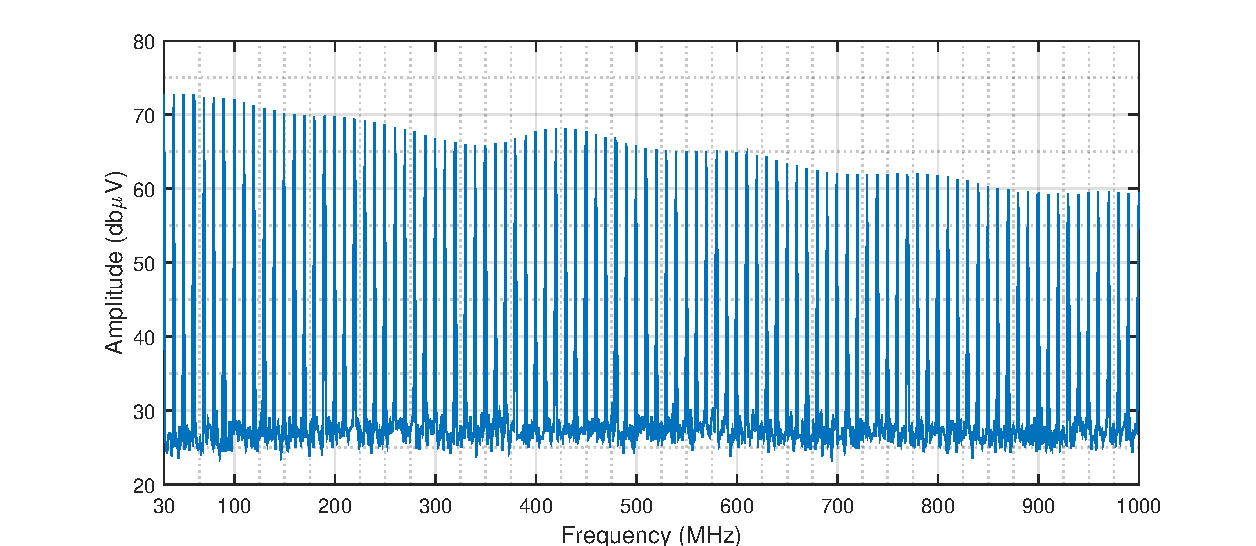
\includegraphics[width=1\columnwidth,draft=false]{comb_re_direct_1.pdf}}
	\caption{Frequency spectrum measured directly from the board RF output}
	\label{fig:comb_re_direct}
\end{figure}

% Figure: Frequency spectrum scan in 3m SAC
\begin{figure}[h]
	\centerline{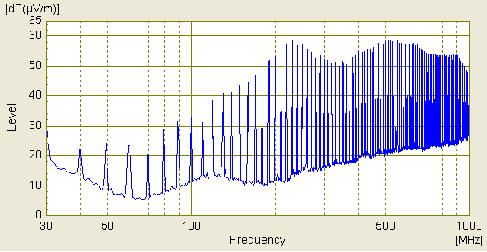
\includegraphics[width=0.9\columnwidth,draft=false]{scan_re_small.pdf}}
	\caption{Field strength measured in 3m semi anechoic chamber}
	\label{fig:scan_re_small}
\end{figure}


% 2x2 figures of radiation patterns
\begin{figure}[ht] 
	\begin{subfigure}[b]{0.5\linewidth}
		\centering
		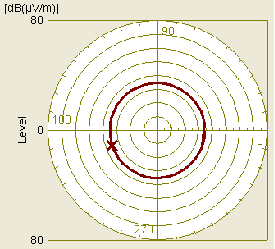
\includegraphics[width=0.75\linewidth]{pattern_100_MHz.pdf} 
		\caption{Radiation pattern at 100 MHz} 
		\label{fig:rad_patt_100} 
		\vspace{4ex}
	\end{subfigure}%% 
	\begin{subfigure}[b]{0.5\linewidth}
		\centering
		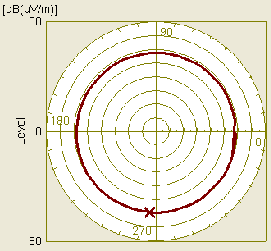
\includegraphics[width=0.75\linewidth]{pattern_230_MHz.pdf} 
		\caption{Radiation pattern at 230 MHz} 
		\label{fig:rad_patt_230} 
		\vspace{4ex}
	\end{subfigure} 
	\begin{subfigure}[b]{0.5\linewidth}
		\centering
		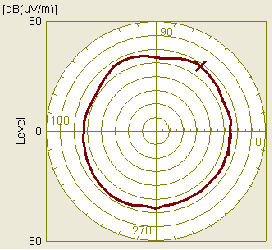
\includegraphics[width=0.75\linewidth]{pattern_800_MHz.pdf} 
		\caption{Radiation pattern at 800 MHz} 
		\label{fig:rad_patt_800} 
	\end{subfigure}%%
	\begin{subfigure}[b]{0.5\linewidth}
		\centering
		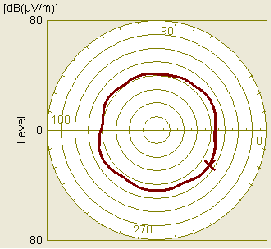
\includegraphics[width=0.75\linewidth]{pattern_970_MHz.pdf} 
		\caption{Radiation pattern at 970 MHz} 
		\label{fig:rad_patt_970} 
	\end{subfigure} 
	\caption{Radiation patterns at various frequencies}
	\label{fig:rad_patt_all} 
\end{figure}

\section{Conclusions}

A simple radiated comb generator has been designed and implemented. It comprises a circular-shaped pulse generator board and a monopole copper rod antenna. It has a unique design in which the pulse former is implemented using PECL DFF. The working principle is exploiting on the asynchronous reset mechanisms of the D Flip-Flop. Although this method is much less explored compared to other methods, such as SRD, Schottky diodes, NLTL, etc., it however shows good performance up to 1000 MHz frequency range. Using crystal oscillator, its frequency accuracy was measured +24 ppm. This can be improved by using more accurate oscillators, such as TCXO and OCXO.  

\ack

The authors would like to thank all the team members of EMC laboratory and electrical laboratory of P2SMTP--LIPI for their support during the project. Big thanks are also addressed to Windi Kurnia P. of Research Center for Metrology (P2M--LIPI) for his assistance in measuring the board pulse output.  



\bibliographystyle{ieeetr}
\bibliography{library}

%\begin{thebibliography}{99}
%\bibitem{article} Lastname,~F.~M., ``Title of the journal paper," {\it Journal Title Abbreviation\/}, Vol.~34, No.~10, 1064--1076, 2013.

%\bibitem{book} Lastname,~F.~M., {\it Book Title \/}, Publisher, City Name, 2014.
%\end{thebibliography}

\end{document}
